\documentclass{article}

\usepackage[textwidth=5.5in,textheight=9.5in]{geometry}
\usepackage{amsmath}
\usepackage{graphicx}
\usepackage{minted}

\title{Particle Physics Project - Pionic Atoms}
\author{Muhammad Sadegh Esmaeilian}
\date{January 2020}

\begin{document}

\maketitle

\section{Overview}
The charmonium system was discovered in November 1974, when two experimental groups at Brookhaven and SLAC announced almost simultaneously the discovery of a new, narrow resonance, later to be called \(\frac{J}{\psi}\).
The well-knowns charmonium systems are listed below with their masses.

\begin{center}
\begin{tabular}{ c | c c }
& $Mass(GeV)$ & $J^{PC}$ \\
\hline 
$\eta_{c}(1s)$ & $2.98$ & $0^{-+}$\\  
$\eta_{c}(2s)$ & $3.64$ & $0^{-+}$\\
$\frac{J}{\psi}(1s)$ & $3.10$ & $1^{--}$\\
$\psi(2s)$ & $3.69$ & $1^{--}$\\
$\psi(4040)$ & $4.04$ & $1^{--}$\\
$\psi(4160)$ & $4.16$ & $1^{--}$\\
$h_{c}(1P)$ & $3.53$ & $1^{+-}$\\
$\chi_{c0}(1P)$ & $3.42$ & $0^{++}$\\
$\chi_{c1}(1P)$ & $3.51$ & $1^{++}$\\
$\chi_{c2}(1P)$ & $3.56$ & $2^{++}$\\
$\chi_{c2}(3930)$ & $3.93$ & $2^{++}$
\end{tabular}
\end{center}

In fact at short antiquark distances \(r < 0.1 fm\), the interaction is dominated by one-gluon exchange that we can write as 

\begin{equation}
	V(r)=-\frac{a(h c)}{r}
\end{equation}
where a is proportional to the strong interaction analogue of the fine structure constant \(\alpha\) in QED. Because of asymptotic freedom, the strength of the interaction decreases with decreasing \(r\), but for \(r < 0.1 fm\) this variation is slight and can in many applications be neglected.
In strong interactions we also have to take account of the fact that the quarks are confined.
The latter part of the potential cannot at present be calculated from QCD and several forms are used in phenomenological applications. All reasonable forms are found to give very similar results for the region of interest. If we choose a linear form, then
\begin{equation}
	V(r)=\frac{b r}{\hbar c}
\end{equation}
This is an example of a confining potential, in that it does not die away with increasing separation and the force between the quark and antiquark cannot be neglected, even when they are very far apart. The full potential is thus
\begin{equation}
	V(r)=-\frac{a(h c)}{r}+\frac{b r}{\hbar c}
\end{equation}
it found that a good fit to both sets of energy levels can be obtained for the same values \(a \approx 0.48\) and \(b \approx 0.18\) GeV.

\section{Solving Schrodinger Equation}
Now that we have form of potential so our job is easy. Because that we have a spherical symmetry in our potential we can seperate the radial part of the equation from the spherical part of it so the radial part may look like this
\begin{equation}
-\frac{\hbar^{2}}{2 M} \frac{d^{2}}{d r^{2}}\left(r R_{n l}(r)\right)+ V(r)+\frac{l(l+1) \hbar^{2}}{2 M r^{2}}\left(r R_{n l}(r)\right)=E_{n}\left(r R_{n l}(r)\right)
\end{equation}
and the spherical parts are the spherical harmonics. Using the second order centered derivative formula we can change this to a eigen-value problem. By writing hamiltonian as a matrix, we should obtain the eigen values which are the energies and the eigen functions are the wave functions. By doing so, our code would looks like this

\begin{minted}
[
frame=lines,
framesep=2mm,
baselinestretch=1,
fontsize=\footnotesize,
linenos
]
{python}
### definig charmonium system potential
def V(i):
    return -a*h_bar*c/(delta_r*i+1e10) + b*(delta_r*i+1e10)/h_bar/c

### definig a function to solve schrodinger equation (with eigen-value problem)
def SH_eq(N, l):
	H = np.zeros([N,N])
	H[0][0] = alpha/delta_r**2 + V(0) + alpha*l*(l+1)/(delta_r)**2
	H[N-1][N-1] = alpha/delta_r**2 + V(0) + alpha*l*(l+1)/(delta_r)**2
	H[0][1] = -alpha/delta_r**2
	H[N-1][N-2] = -alpha/delta_r**2

	for i in range(1,N-1):
	    H[i][i-1] = -alpha/delta_r**2
	    H[i][i] = 2*alpha/delta_r**2 + V(i) + alpha*l*(l+1)/(delta_r*i)**2
	    H[i][i+1] = -alpha/delta_r**2

	return H
\end{minted}
By doing so and running the code, it is time to compare results with data about their energies. The real energies are
\begin{figure}[h]
    \includegraphics[width=8cm]{B.png}
    \centering
\end{figure}
The energies of my calculations are listed below
\begin{center}
\begin{tabular}{ c | c }
Charmonium& $Energy/(c^{2})(GeV/(c^{2})$ \\
\hline 
$\eta_{c}(1s)$ & $-98.42$\\  
$\eta_{c}(2s)$ & $568.65$\\
$\frac{J}{\psi}(1s)$ & $5.23$\\
$\psi(2s)$ & $608.29$\\
$\psi(4040)$ & $936.51$\\
$\psi(4160)$ & $1046.19$\\
$h_{c}(1P)$ & $462.82$\\
$\chi_{c0}(1P)$ & $330.42$\\
$\chi_{c1}(1P)$ & $426.51$\\
$\chi_{c2}(1P)$ & $472.56$\\
$\chi_{c2}(3930)$ & $831.93$
\end{tabular}
\end{center}
Now by plotting this we get 
\begin{figure}[h]
    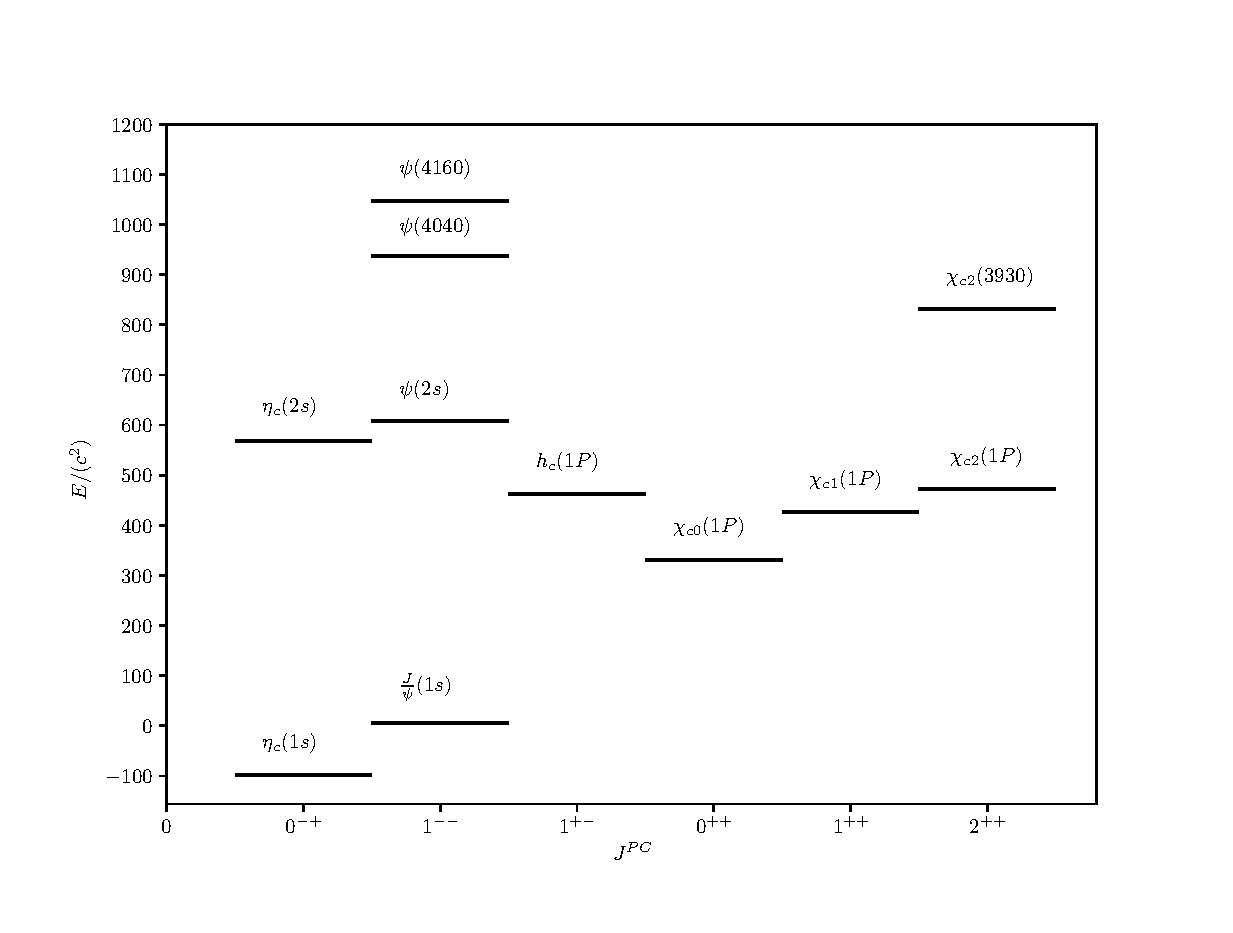
\includegraphics[width=10cm]{CH.eps}
    \centering
\end{figure}

which is almost similar to the above plot that is from real data.
\end{document}